\documentclass[man,noapacite]{apa2}
\usepackage{amsmath}
\usepackage{booktabs}
\usepackage{apacite2}
\usepackage{fullpage,rotating}
\usepackage{pslatex}
\usepackage{amssymb}
\usepackage{accents}

% \usepackage{synctex}

\newcommand{\vect}[1]{\accentset{\rightharpoonup}{#1}}

\title{Learning word meaning by inferring speakers' intentions: \\ An incremental approach to socially-guided statistical learning}

\threeauthors{Michael C. Frank}{Molly L. Lewis}{Noah D. Goodman}
\threeaffiliations{Department of Psychology, Stanford University}{Department of Psychology, Stanford University}{Department of Psychology, Stanford University}

\shorttitle{Learning words by inferring reference}
\rightheader{Learning words by inferring reference}


\acknowledgements{Many thanks to ...

~

\noindent Please address correspondence to Michael C. Frank, Department of Psychology, Stanford University, 450 Serra Mall (Jordan Hall), Stanford, CA, 94305, tel: (650) 724-4003, email: \texttt{mcfrank@stanford.edu}.}


\abstract{How do children learn the meanings of words? While some accounts suggest that word learning happens in a single moment, others privilege the gradual accumulation of information across time. Previous modeling work has attempted to unify these viewpoints in a single framework that allows for both in-the-moment interpretation and gradual statistical accumulation, but at the cost of substantial computational complexity. We describe a new, incremental model of this interaction, in which statistical associations are the product of in-the-moment interpretations. This process-level model successfully captures a number of experimental findings (including some that were not captured by previous, computational-level analyses) and suggests a number of extensions.}

\begin{document}
\maketitle                            


\section{Introduction}

How do children learn their first words? 


\subsection{Prior modeling work}

Early work on modeling cross-situational word learning. 
An important cross-situational word learning was proposed by \citeA{siskind1996}; this model used a propositional representation of meaning in combination with a set of deductive rules to infer word-meaning mappings from artificial data. This ambitious model provided a powerful proof-of-concept, but was limited by the assumption that the propositional structure of meanings was observed by the learner. 

\subsection{The current paper}


\section{Modeling details}

\subsection{Model Specification}
\begin{figure}[tr]
\begin{center}
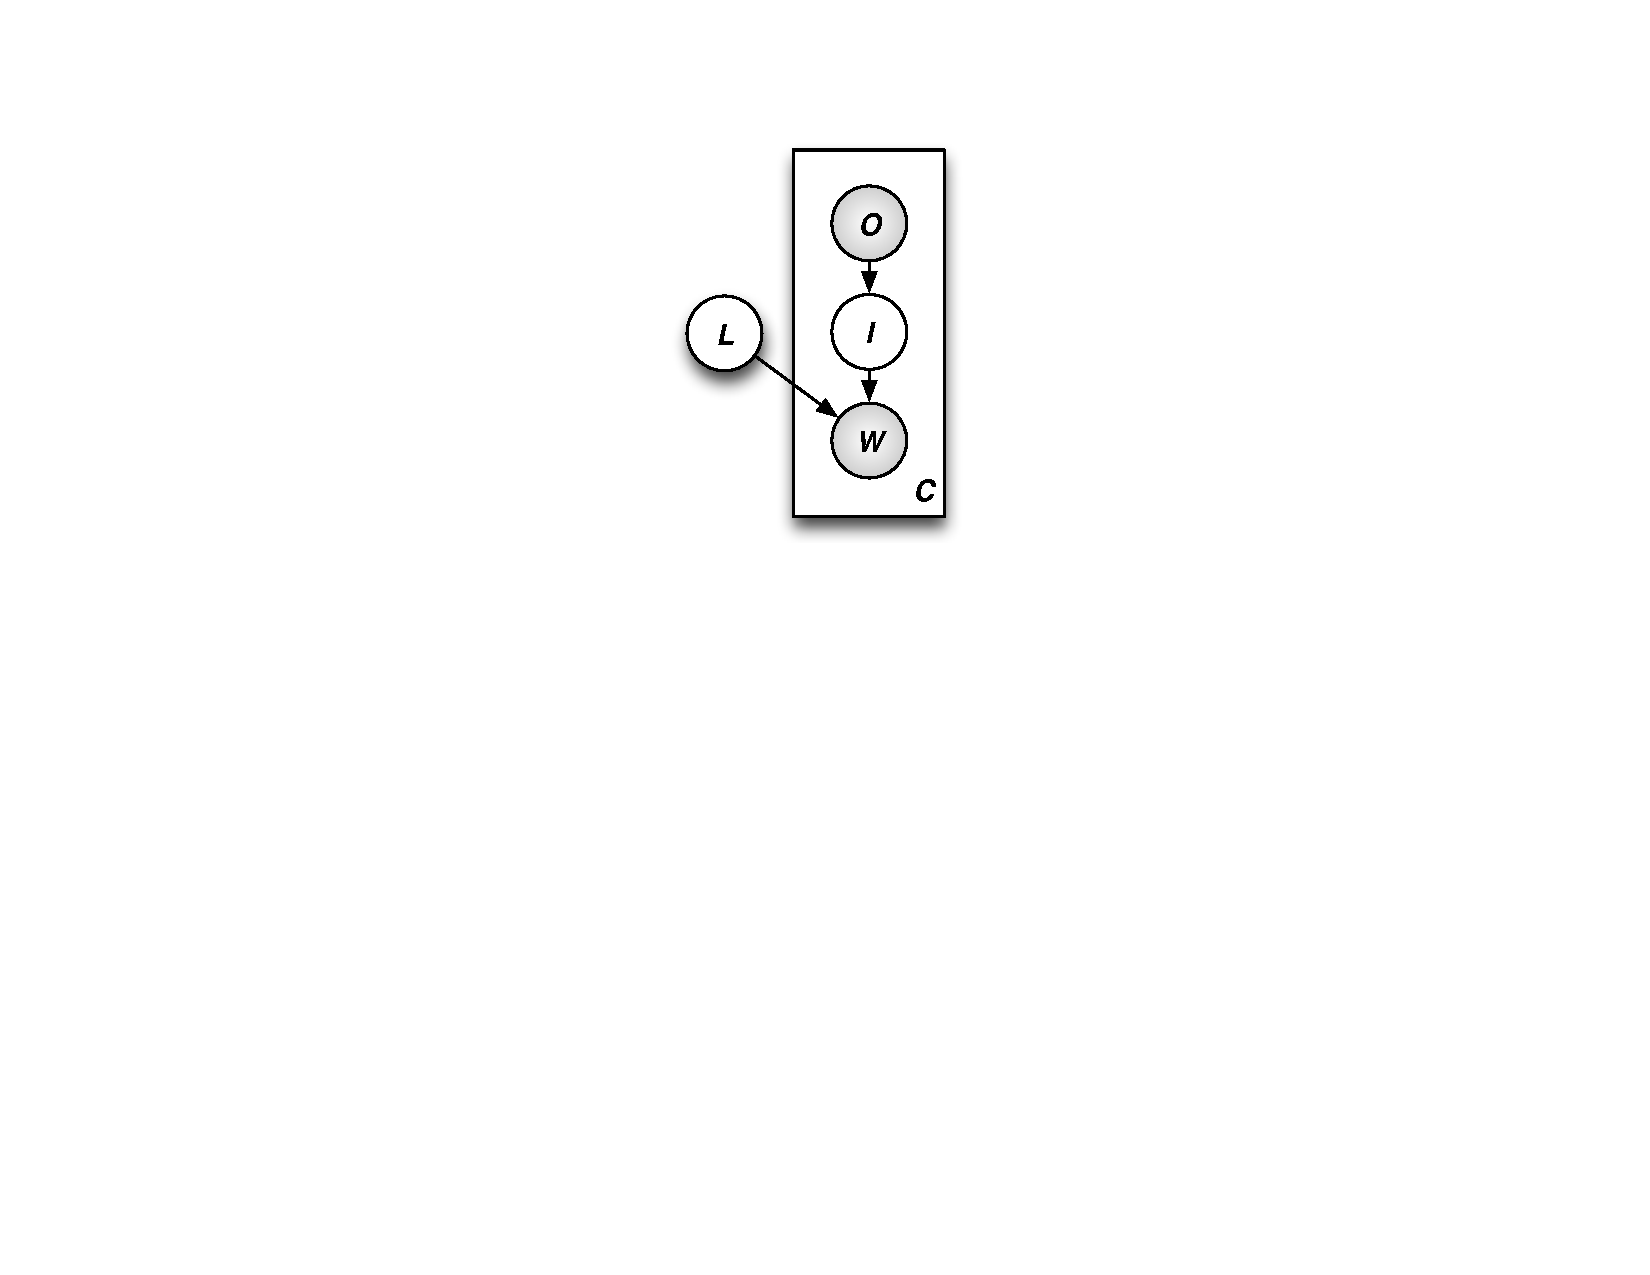
\includegraphics[width=1.5in]{figures/gen_mod.pdf}
\caption{\label{fig:genmod} Caption.}
\end{center}
\end{figure}

\begin{figure}[tr]
\begin{center}
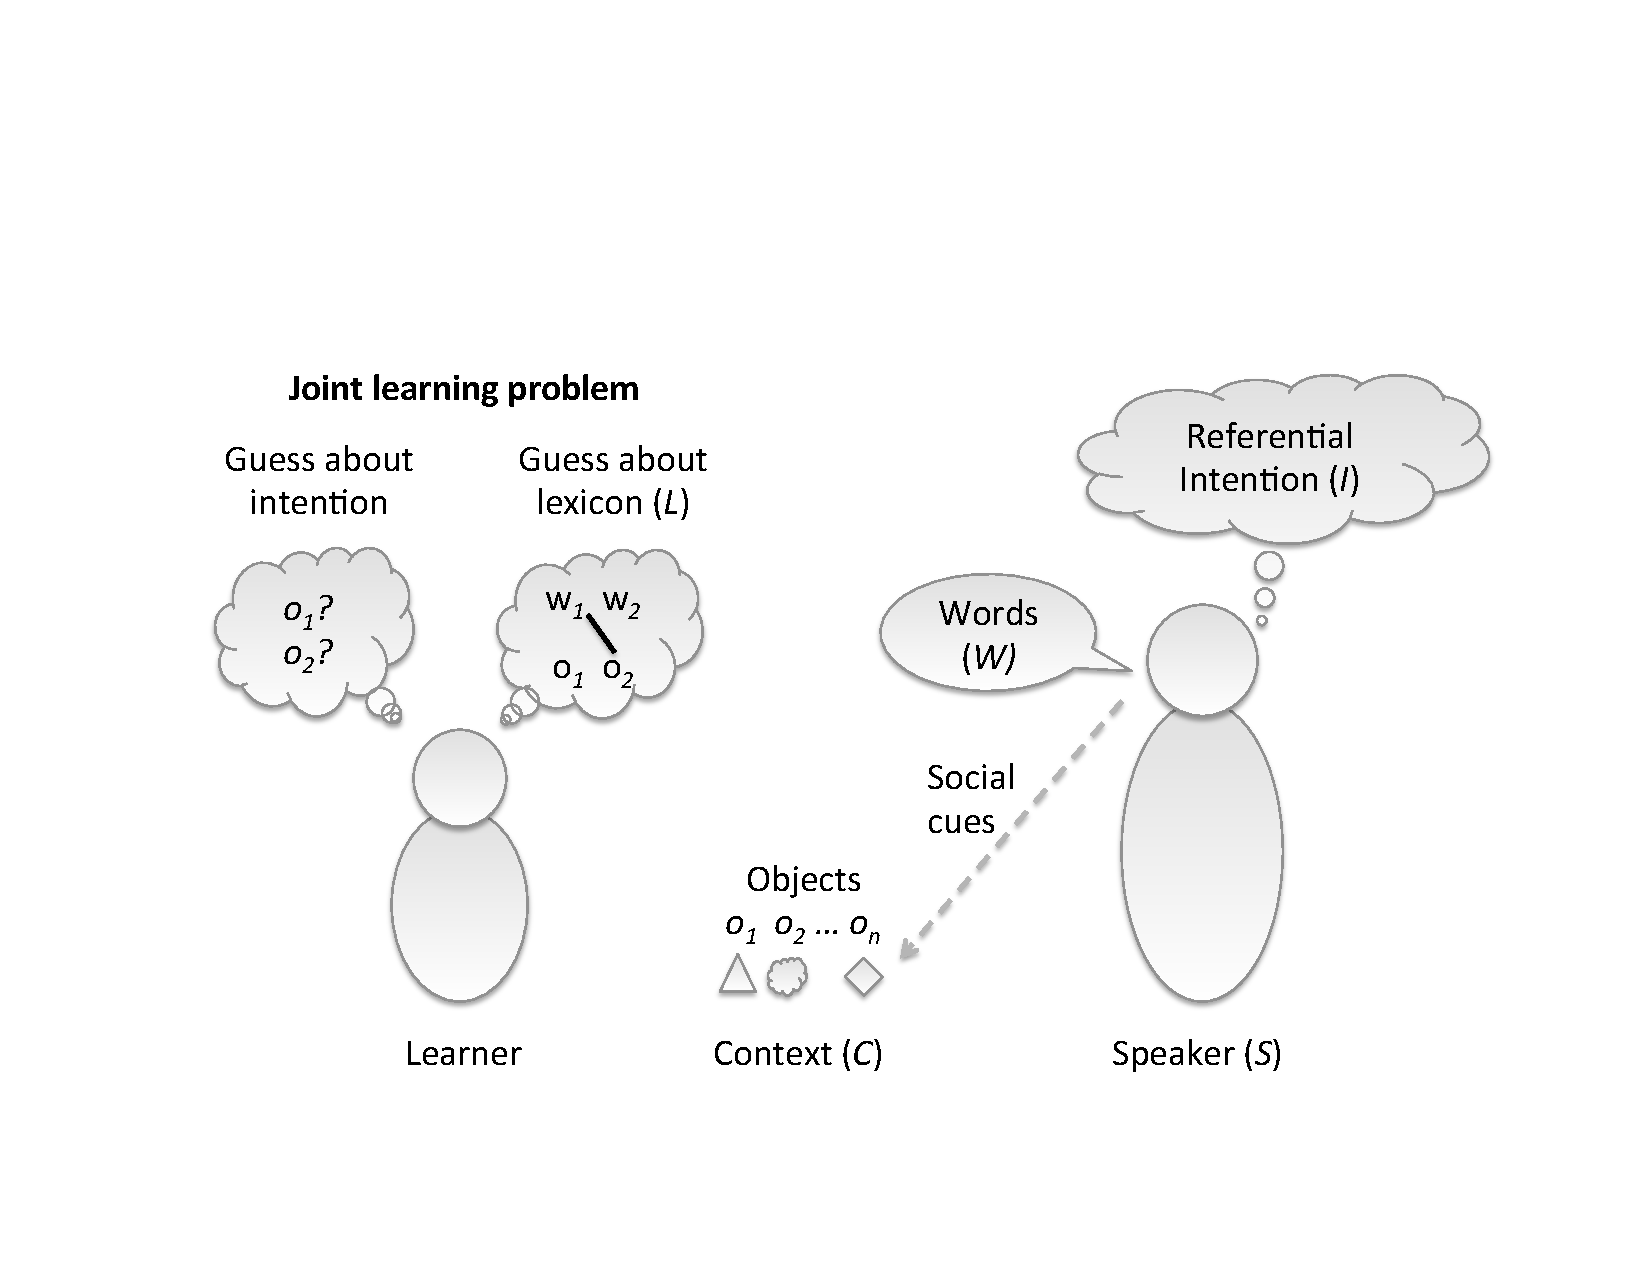
\includegraphics[width=4.5in]{figures/setup.pdf}
\caption{\label{fig:setup} Caption. From Frank (in press). }
\end{center}
\end{figure}

By Bayes' rule:

\begin{equation}
P( I, L | C) \propto P(C | I, L ) P(I, L).
\end{equation}


% \begin{equation}
% P( I| W, O) \propto P(W | I, O) P(I).
% \end{equation}

\begin{equation}
P( I, L | W, O) \propto P(W, O | I, L) P(I, L).
\end{equation}


\noindent But the objects $O$ are observed in the context. In addition, for simplicity, we assume that there is a uniform prior over possible intentions (though we return to this issue in the Discussion). By the generative model in Figure \ref{fig:genmod}, the remaining expression can be factored as follows:

\begin{equation}
P( I, L | W, O) \propto P(W | I, L) P(I | O) P(I) P(L).
\end{equation}

But now we integrate over all possible L:

\begin{equation}
P( I| W, O) \propto \int_L{P(W | I, L) P(I | O) P(I)  P(L) }
\end{equation}


In this model, the lexicon $L$ consists of two separate parts. The referential lexicon $L_R$ is a set of integrated Dirichlet-Multinomial distributions, one for each object in the world. This distribution represents the posterior probability of a particular word, relative to that object. 

\begin{equation}
P(L) = \prod_{o \in W}{P(L_{R_o})} + P(L_{NR}).
\end{equation}

 

% \begin{equation}
% P(W | I, L) = \gamma  
% \end{equation}

% intention, referential slot, and word vector
% for the referential word 

$p(\vect{w} | I, R, L_R, L_{NR}) = p(w|O_i) * prod_{s \in S - S_r} {P(W_s | L_{NR})}$

\subsection{Inference}
\begin{figure}[tr]
\begin{center}
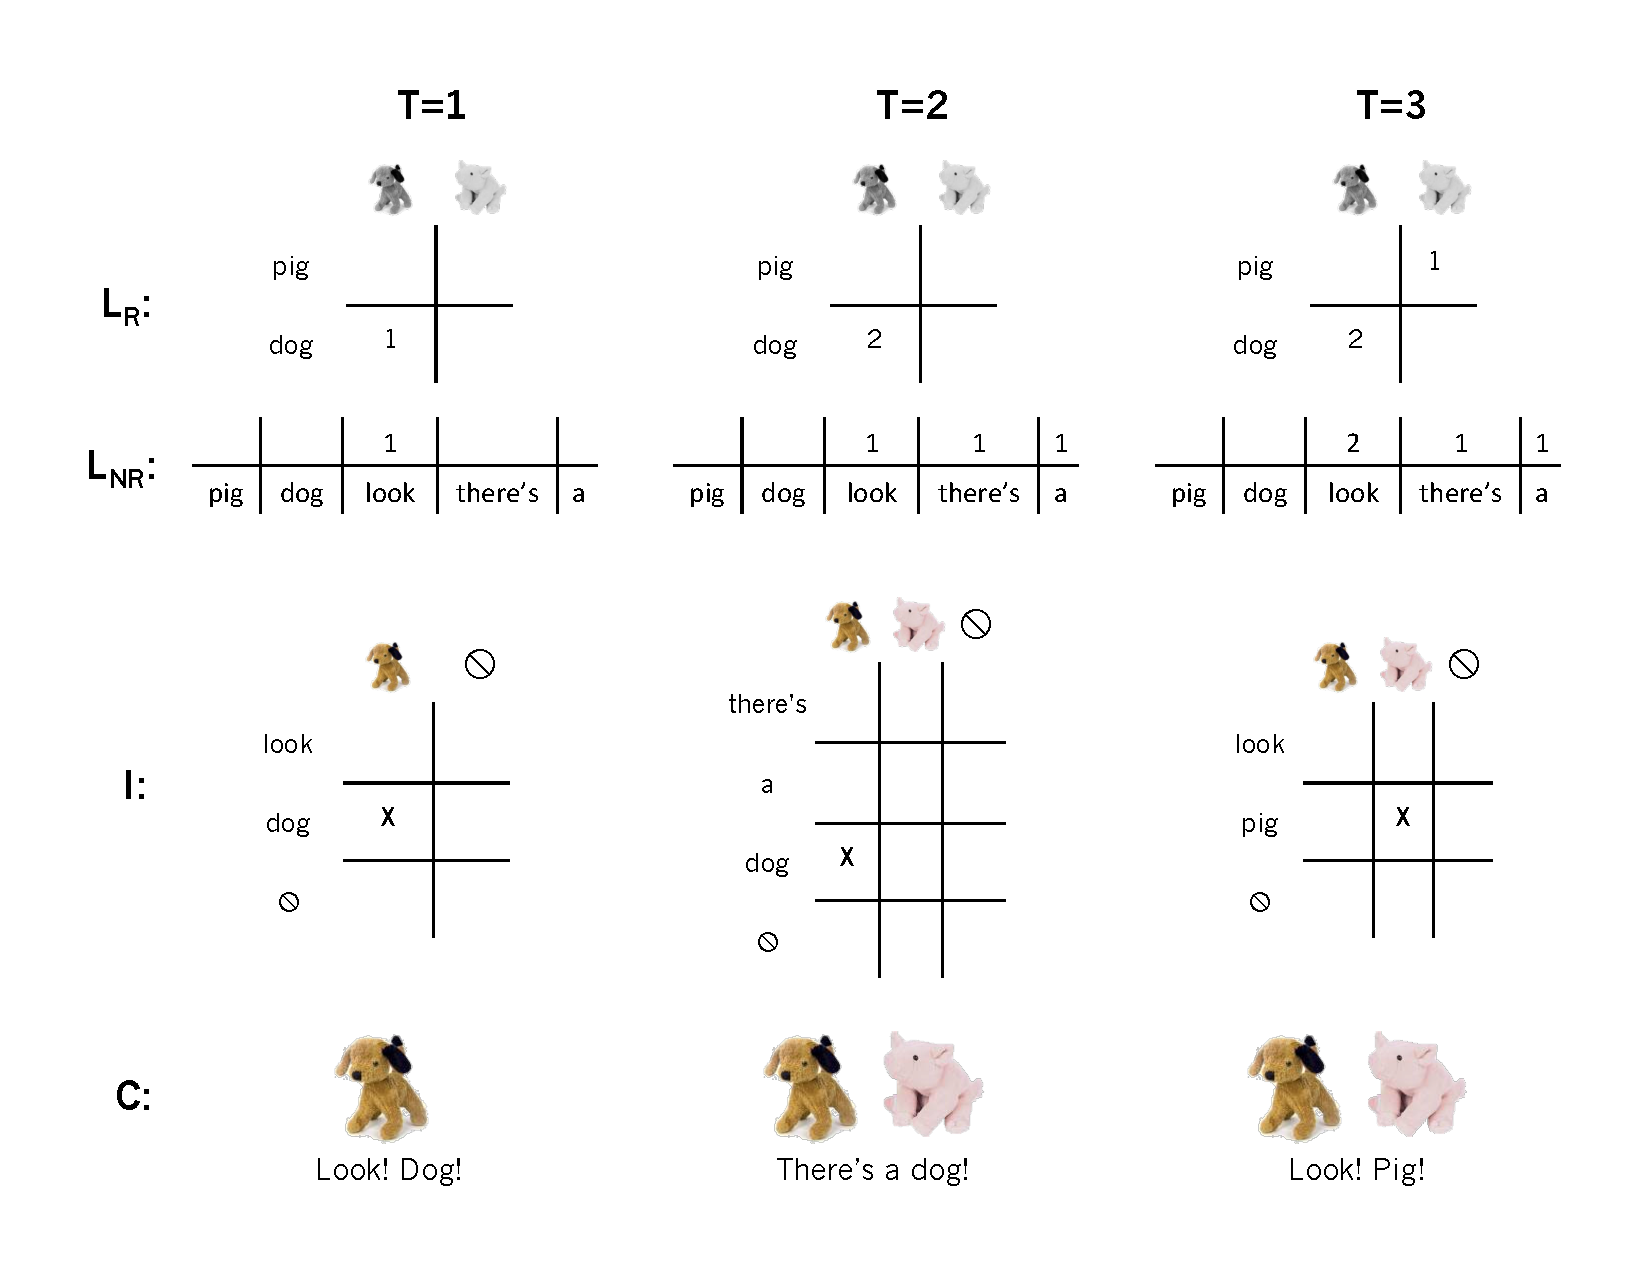
\includegraphics[width=6.5in]{figures/inference_diagram.pdf}
\caption{\label{fig:inference_diagram} Caption.}
\end{center}
\end{figure}

\subsubsection{Batch inference using a gibbs sampler}

\begin{equation}
P_t(L|W_{1...t}, O_{1...t}) \propto P_{t-1}(L | ...) P(W_t, I_t, R_t | L)
\end{equation}

% prob of a particular sample under Dir-M is the same thing as the conjugate 
% so you just get the conjugate update for each of the assignments 

\subsubsection{Incremental inference using a particle filter}

\begin{equation}
P_t(L|W_{1...t}, O_{1...t}) \propto P_{t-1}(L | ...) P(I_t | W_t, O_t)
\end{equation}

\section{Simulations}

\subsection{Cross-situational word learning with adults}

\subsubsection{Yu \& Smith (2007)}

\subsection{Experiments with children}

\subsubsection{Disambiguation}

\subsubsection{Dewar \& Xu (2007)}


\subsection{Corpus simulations}

\subsection{Rollins subset (Frank, Goodman, \& Tenenbaum, 2009)}

\subsection{Fernald \& Morikawa (Johnson, Demuth, \& Frank, 2012)}

\section{Discussion}

\newpage

\bibliographystyle{apacite}
\bibliography{icom}

\end{document}

